%\chapter{Introduction}
\chapter[Introduction]{Introduction
\footnote{
  $CVS~revision~ $Id: a-intro.tex,v 1.7 2008/04/01 16:50:02 lerose Exp $ $ 
}
\footnote{Authors: J.LeRose \email{lerose@jlab.org} and
                   E.Chudakov \email{gen@jlab.org}}
}
\ifpdfhref{ 
\section[About this Document]{Technical Information About this Document}
\label{sec:intro-about}
 {\it
 This is a PDF document with hyper-references. Browsing is helped
 by the ``bookmark'' menu at the left side of the \mycomp{acroread} or
 \mycomp{xpdf} window. 
% Another browser, \mycomp{xpdf} seems to lack this option.
 The objects like
 citations, figures, tables etc. are hyper-marked. One can ``click''
 on a reference to an object and jump to the page with this
 object. Jumping back can be done using the right mouse button (\mycomp{acroread})
 or the left arrow button at the bottom of the window (\mycomp{xpdf}).
 External references to the Web are also ``clickable''.
 In order to use them, make sure that your PDF browser is configured
 to work with a Web browser (use the button ``Preferences'' in \mycomp{acroread},
 or provide and edit the file \mycomp{$\tilde{}$/.xpdfrc} for \mycomp{xpdf}).
 One should open a Web browser window and afterward one may
 use the WWW-links from the PDF browser. Finally, the PDF browsers
 allow to search for a given pattern in the whole document. 

 The areas of text, dedicated to
 safety issues, are marked by red color throughout this document.
 Sometimes only the titles of the appropriate sections are marked.
 Also, red margin bars mark the beginnings of these areas.
 
 \LaTeX{} (more specifically, \mycomp{pdflatex}) is used to produce
 this document. The document source is kept in CVS~\cite{CVSwww} format\footnote{
   Instruction for the document authors/maintainers: 
   \url{http://www.jlab.org/~gen/osp/doc.pdf}.}.

 Typically, each chapter or a big section occupies one file,
 and the date of CVS revision of the file is printed
 in a footnote for the chapter title, along with the name of
 the author or the person responsible for the chapter.\\

 This document can be printed, but it is better used on-line.
}
\clearpage
}

\section[Purpose]{The Purpose of this Document}
\label{sec:intro-purpose}

 This document contains the following information concerning the Hall
 A ``base equipment'':
 \begin{list}{--}{\setlength{\itemsep}{-0.2cm}}
    \item general overview; 
    \item safety assessment; 
    \infolevone{\item technical overview;} 
    \infolevtwo{\item operating procedures;} 
    \infolevthree{\item performance information.}
 \end{list}

\noindent{}The requirements to Hall A personnel training 
are outlined in Sec.~\ref{sec:access-req}. 
Although reading of this OSP document is not explicitly required, 
the other documents refer to it, as far as
safe operations of the base Hall A equipment are concerned.\\

\infolevtwo{
  The operating procedures are intended to
  provide shift personnel with the information they need to
  understand, at least at a rudimentary level, the function of the
  various subsystems in the end-station. It should also aid in
  determining if the equipment is performing properly and provide
  instructions for what to do in the case of malfunctions. This
  document does not necessary give a complete comprehensive reference 
  to each subsystem, but at least provides a guide for the shift 
  personnel. When appropriate,
  other references are indicated for the user who requires more
  information.  \\

  A reduced version of this document is available\cite{HallAosp0},
  which contains the Safety Assessment part of the document (SAD) along
  with only very general description of the components.
}

 A comprehensive description of the equipment performance in given
 in a published paper~\cite{HallA-NIM}. 
\infolevtwo{
 This OSP includes some
 information on this matter in order to help the shift workers
 to check up the equipment.
}

\infolevltthree{
\begin{safetyen}{10}{15}
 This is primarily the Safety Assessment Document (SAD) along with
 a reduced version ({\it ``info level \infolevel{}''}) of the OSP document. 
 It is sufficient to get acquainted with the basic equipment and the general safety
 measures, but might not be sufficient to operate a given component 
 of the equipment. For operation one should read the full ({\it ``info level 4''}) 
 OSP document~\cite{HallAosp}.  
\end{safetyen}
}
\clearpage
\section[Hall A Overview]{Hall A Overview}
\label{sec:intro-halla-overview}

The design purpose of Hall A is to study electron scattering 
on nuclei and nucleons at high luminosity
of up to $5\cdot{}10^{38}~\mathrm{cm^{-2}s^{-1}}$ with high momentum
resolution. The ($e,e^{\prime}p$) reaction is often utilized.
The spectrometers must have high resolution 
to be able to isolate the different reaction channels in nuclei.

The basic lay-out of Hall A is shown in Fig.~\ref{fig:HallA-side},
demonstrating the Hall dimensions.
\infolevtwo{A CAD-drawn 3-dimensional view of the Hall 
is given on the scalable picture on the \hyperlink{pict:cover}{cover} page.}

\begin{figure}[htb]
 \begin{center}
    \includegraphics*[angle=0,width=\textwidth]{HallA}
 \end{center}
\caption[Hall A schematic cross section]%
{Schematic cross section of Hall A with one of the HRS 
spectrometers in the (fictitious) 0$^\circ$ position. 
}
\label{fig:HallA-side}
\end{figure}

The beam line transports the CEBAF electron beam, in the energy 
and current ranges of 0.4~-~6.0~GeV and 0.1~-~120~$\mu$A to the target
at the Hall center. Various types of targets have been used, including
liquid hydrogen and polarized $^3$He gas. Secondary particles
are detected with the  
two High Resolution Spectrometers (HRS). Both of these devices  
provide a momentum resolution of better than $2\times 10^{-4}$ and a horizontal angular 
resolution of better than 2 mrad at a design maximum central momentum 
of 4 GeV/$c$. The rest of the beam is transported to the high power
water cooled beam dump.

The present base instrumentation in Hall A has been used with great 
success for experiments which require high luminosity and high resolution 
in momentum and/or angle for at least one of the reaction products.
	
%\infolevthree{  
%  A CAD-drawn view of Hall A and its basic equipment is shown
%  on Fig.\ref{fig:cad_halla_1}.
%\begin{figure}[tbh]
%\begin{center}
%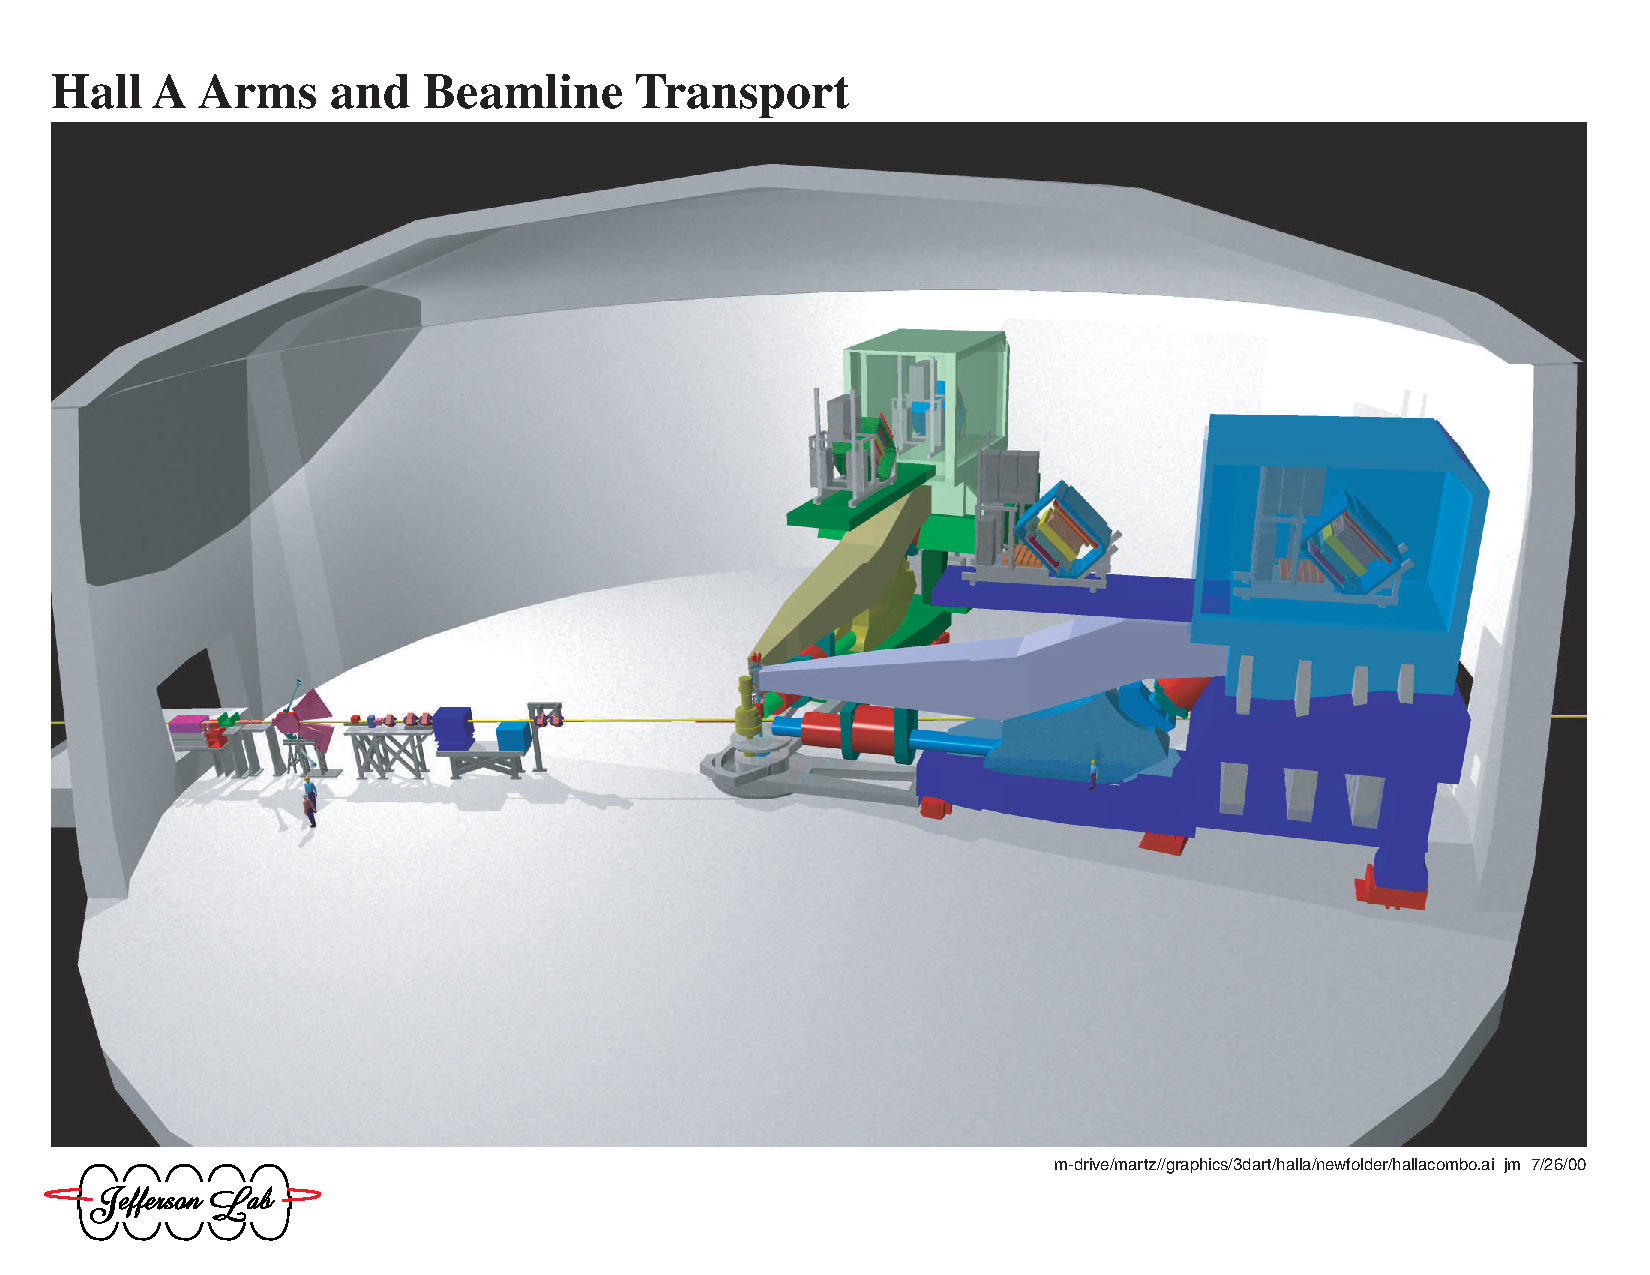
\includegraphics[angle=0,width=\textwidth]{hallacombo}
%\caption[Hall A CAD-drawn picture]
%   {Hall A CAD-drawn picture.}
%\label{fig:cad_halla_1}
%\end{center}
%\end{figure}
%}
